%File: formatting-instruction.tex
\documentclass[letterpaper]{article}
\usepackage{aaai2026}  % DO NOT CHANGE THIS
\usepackage{times}  % DO NOT CHANGE THIS
\usepackage{helvet}  % DO NOT CHANGE THIS
\usepackage{courier}  % DO NOT CHANGE THIS
\usepackage[hyphens]{url}  % DO NOT CHANGE THIS
\usepackage{graphicx}  % DO NOT CHANGE THIS
\urlstyle{rm}  % DO NOT CHANGE THIS
\def\UrlFont{\rm}  % DO NOT CHANGE THIS
\usepackage{natbib}  % DO NOT CHANGE THIS AND DO NOT ADD ANY OPTIONS TO IT
\usepackage{caption}  % DO NOT CHANGE THIS AND DO NOT ADD ANY OPTIONS TO IT
\frenchspacing  % DO NOT CHANGE THIS
\setlength{\pdfpagewidth}{8.5in}  % DO NOT CHANGE THIS
\setlength{\pdfpageheight}{11in}  % DO NOT CHANGE THIS

\usepackage{amsmath,amssymb,amsthm}
\usepackage{booktabs}

\pdfinfo{
/TemplateVersion (2026.1)
}

\setcounter{secnumdepth}{0}

\title{Replicating SO(2)-Equivariant Reinforcement Learning for Robot Manipulation, with an Extension to ManiSkill}
\author{
    Wade Williams,
    Joseph Horwitz
}
\affiliations{
    Khoury College of Computer Sciences, Northeastern University\\
    CS 5180 Reinforcement Learning, Spring 2026\\
    \{williams.wad, horwitz.jo\}@northeastern.edu
}

\begin{document}
\maketitle

\begin{abstract}
In this project, we implement the $SO(2)$-Equivariant SAC and DQN algorithms published in \citet{wang2022so2} from scratch and reproduce their main results on three PyBullet tasks: block pulling, object picking, and drawer opening. Each equivariant method is compared against the same data-augmentation and contrastive baselines used in the paper (DrQ, FERM, CURL). Equivariant SAC reaches a discounted evaluation reward of $\approx 0.93$ on all three tasks with every non-equivariant SAC baseline staying near zero. Equivariant DQN leads the DQN methods tested on block pulling and object picking, and the gain from equivariance is smaller for DQN than for SAC, matching the results show in the original paper. We then extend the codebase to ManiSkill~3 and run a comparison on PickCube-v1, the closely related ManiSkill task to the paper's object-picking task. Under ManiSkill's default normalized dense reward, the two algorithm variants converge similarly, with the equivariance gain still visible. One extension with more time would be a sparse-reward comparison on ManiSkill at a higher training budget, and a contrastive-pretraining pass for the FERM baseline.
\end{abstract}

% reword
\section{Introduction}
Sample efficiency is a central problem in reinforcement learning as a policy is only useful if it can be learned from a reasonable amount of environmental interaction. This matters especially in robotics, where every sample comes from a physical robot, rollouts cost time, and an unsafe policy can damage the robot or its surroundings. One approach to improving sample efficiency is data augmentation, which refers to creating artificial experiences by applying affine transformations (e.g., image translation or rotation) to the states in a transition \citep{laskin2020rad,kostrikov2020drq}, while other approaches add a contrastive loss \citep{laskin2020curl,zhan2020ferm}.

Geometric deep learning takes a more direct route to the same inductive bias. \citet{cohen2016gcnn,cohen2016steerable} showed that equivariant neural networks can represent transformation-invariant functions by construction. Both approaches target the same bias, but equivariant architectures encode it in the model rather than in the training data. With data augmentation, the model has to learn equivariance alongside the task, which usually costs more training time and more model capacity. Even then, the equivariance is only approximate, while equivariant networks guarantee it exactly and often generalize better \citep{wang2020symmetry}. Early work in equivariant reinforcement learning focused on discrete groups in grid-world and toy domains \citep{vanderpol2020plannable,vanderpol2020mdp,mondal2020group}.

\citet{wang2022so2} scaled the approach to realistic visuomotor manipulation. They showed that $SO(2)$-equivariant networks can achieve substantially better sample efficiency than the standard and data-augmentation baselines on close-loop PyBullet tasks. Their result has been a reference point for later work that extends architectural equivariance to new policy classes and larger symmetry groups, including Equivariant Diffusion Policy \citep{wang2024diffusion}, Spherical Diffusion Policy \citep{spherical2025}, and 3D equivariant visuomotor policies on point clouds \citep{equivariant3d2025}. In this project, we reproduce the main results of \citet{wang2022so2}: Equivariant SAC and Equivariant DQN against the same data-augmentation and contrastive baselines Wang et al.\ used, on three close-loop PyBullet manipulation tasks (block pulling, block picking, and drawer opening). We then extend the comparison to ManiSkill~3, a GPU-parallel manipulation simulator, to see whether the sample-efficiency gain carries over to a different physics backend and camera pipeline.

\section{Related Work}

\subsection{Data Augmentation and Contrastive Learning}
Most work on improving sample efficiency in visuomotor reinforcement learning uses some form of pixel-space data augmentation during training. DrQ \citep{kostrikov2020drq} augments each minibatch with random shifts and averages the Q-target across the augmented copies. RAD \citep{laskin2020rad} applies random crops directly to observations as they enter the actor and critic. Both methods train the encoder to be robust to affine transformations through repeated exposure to augmented samples. A related line of work adds a contrastive objective on top of the augmentation \citep{oord2018cpc}. CURL \citep{laskin2020curl} trains the encoder to pull augmented views of the same observation together in latent space, and FERM \citep{zhan2020ferm} adapts that pipeline to sample-efficient robotic manipulation by combining SAC, random crop, and contrastive pretraining. Wang et al.\ compare against these three methods (DrQ, CURL, and FERM) in their paper, and we use this set of baselines in our replication.

\subsection{Equivariant Architectures in Reinforcement Learning}
A separate line of work addresses the same sample-efficiency problem by encoding symmetry directly into the network instead of learning it from data. \citet{cohen2016gcnn,cohen2016steerable} introduced group-equivariant convolutional networks, generalizing the translation-equivariant property of standard CNNs to arbitrary finite symmetry groups. \citet{weiler2019e2cnn} extended this to the Euclidean group $E(2)$ through steerable convolutions, which is the framework both Wang et al.\ and our implementation build on. The first applications of equivariance to reinforcement learning were limited to small discrete symmetries in toy domains: \citet{mondal2020group} used steerable CNNs on two game environments, and \citet{vanderpol2020mdp} proposed MDP homomorphic networks for encoding rotational and reflectional equivariance on a small set of tasks. \citet{wang2021equivariant} was the first to apply the idea to robotic manipulation, but their formulation was restricted to the spatial action space, where the policy outputs a target end-effector pose rather than an incremental displacement. \citet{wang2022so2}, the paper we replicate, was the first to scale architectural equivariance to close-loop manipulation with both discrete (DQN) and continuous (SAC) action spaces, and showed a large sample-efficiency advantage over the augmentation and contrastive baselines at this scale.

\subsection{Extensions Since Wang et al.\ (2022)}
The approach has since been extended along several axes. \citet{wang2022onrobot} ported the same $SO(2)$-equivariant architecture onto a physical UR5 arm and showed that the sample-efficiency gains carry over from simulation to real hardware. Later work has generalized both the symmetry group and the policy class. Equivariant Diffusion Policy \citep{wang2024diffusion} combines $SO(2)$-equivariant backbones with diffusion policy heads on MimicGen. Spherical Diffusion Policy \citep{spherical2025} extends this to the full $SE(3)$ Euclidean group through spherical CNNs. Other work applies equivariance to related manipulation components, including grasp-pose prediction with Equivariant Descriptor Fields \citep{ryu2023edf} and 3D visuomotor policy learning from point clouds \citep{equivariant3d2025}.


\section{Background}

\subsection{Soft Actor-Critic}
Soft Actor-Critic (SAC; \citealp{haarnoja2018sac}) is the off-policy actor-critic algorithm we use for our continuous-action agents. SAC maximizes an entropy-regularized return
\begin{equation}
J(\pi) = \mathbb{E}_{\tau \sim \pi}\!\left[ \sum_{t=0}^{\infty} \gamma^{t} \big( r_t + \alpha \, \mathcal{H}(\pi(\cdot \mid s_t)) \big) \right],
\end{equation}
where $\alpha$ is an automatically tuned temperature and $\mathcal{H}$ is the policy entropy. It trains twin $Q$-networks $Q_{\phi_1}, Q_{\phi_2}$ against the soft Bellman target
\begin{equation}
y = r + \gamma \left( \min_{i} Q_{\bar\phi_i}(s', a') - \alpha \log \pi_\theta(a' \mid s') \right),
\end{equation}
a stochastic Gaussian actor $\pi_\theta$ that minimizes $\mathcal{L}_\pi = \mathbb{E}\big[ \alpha \log \pi_\theta(a \mid s) - \min_i Q_{\phi_i}(s, a) \big]$, and target networks $Q_{\bar\phi_i}$ updated by Polyak averaging at rate $\tau$. The twin critics reduce Q-value overestimation, and the entropy bonus encourages exploration.

\subsection{Deep Q-Networks}
Deep Q-Networks (DQN; \citealp{mnih2015dqn}) is the off-policy value-based algorithm we use for our discrete-action agents. DQN fits a single $Q$-network $Q_\phi$ against the greedy Bellman target
\begin{equation}
y = r + \gamma \max_{a'} Q_{\bar\phi}(s', a')
\end{equation}
under a Huber loss, with target network $Q_{\bar\phi}$ updated by Polyak averaging at rate $\tau$. Our equivariant agents inherit these SAC and DQN losses unchanged. The paper's contribution is entirely in the network architectures that realize $\pi_\theta$ and $Q_\phi$.

\subsection{Equivariant Neural Networks}
A function $f \colon X \to Y$ is \emph{equivariant} with respect to a group $G$ acting on $X$ and $Y$ if $f(g \cdot x) = g \cdot f(x)$ for every $g \in G$ and $x \in X$, and \emph{invariant} if $f(g \cdot x) = f(x)$. Invariance is a special case of equivariance in which the action on $Y$ is trivial. For top-down robotic manipulation, the relevant group is $SO(2)$, the group of planar rotations of the workspace: rotating the world and the gripper by the same angle gives the same task. Equivariant convolutional networks approximate $SO(2)$ with its cyclic subgroup $C_n = \{2\pi k/n : k = 0, \dots, n-1\} \subset SO(2)$, a finite group of $n$ evenly-spaced rotations.

The action of $g \in C_n$ on a feature map depends on the \emph{representation} chosen for the map, which specifies how the channel values change when the spatial dimensions rotate. Three representations are used in the agents we build. The \emph{trivial representation} $\rho_0$ leaves channel values unchanged under rotation, which fits scalar quantities such as a depth value at a pixel. The \emph{standard representation} $\rho_1$ is the natural action of $C_n$ on $\mathbb{R}^2$: a two-channel feature $v$ transforms as $\rho_1(g) v = R_g v$, which fits a planar vector such as the $(a_x, a_y)$ component of an action. The \emph{regular representation} $\rho_\text{reg}$ acts on $n$-channel features by cyclically permuting the channels, and is the default representation inside the hidden layers of the equivariant networks.

An equivariant convolutional layer $h$ is built so that rotating the input feature map through any $g \in C_n$ rotates the output by the same group element:
\begin{equation}
h(g \cdot \mathcal{F}_\text{in}) = g \cdot h(\mathcal{F}_\text{in}).
\end{equation}
\citet{weiler2019e2cnn} show that this reduces to a linear condition on the convolutional kernel, and their \texttt{e2cnn} library provides these layers as drop-in replacements for ordinary convolutions. A network built entirely from equivariant layers is itself equivariant by composition, so the equivariance is enforced by the weights themselves regardless of training data. Applying this idea to reinforcement learning goes back to an older result: MDPs with group symmetries have optimal solutions with the same symmetries \citep{ravindran2001symmetries,vanderpol2020mdp}. The next section reviews the specific version of that result developed by \citet{wang2022so2}, which is what motivates the architectures of Equivariant SAC and Equivariant DQN.


\section{Group-Invariant MDPs}

\citet{wang2022so2} formalize the connection between group symmetry and reinforcement learning through what they call a \emph{group-invariant MDP}. Consider a discounted MDP $\mathcal{M} = (\mathcal{S}, \mathcal{A}, P, R, \gamma)$ and a group $G$ that acts on both $\mathcal{S}$ and $\mathcal{A}$. The MDP is \emph{$G$-invariant} if the transition distribution and the reward function are both preserved by the group action:
\begin{align}
P(g \cdot s' \mid g \cdot s, g \cdot a) &= P(s' \mid s, a), \\
R(g \cdot s, g \cdot a) &= R(s, a),
\end{align}
for every $g \in G$. Under this assumption, \citet[Section~4]{wang2022so2} prove that the optimal $Q$-function is itself $G$-invariant and the optimal policy is $G$-equivariant:
\begin{align}
Q^*(g \cdot s, g \cdot a) &= Q^*(s, a), \\
\pi^*(g \cdot s) &= g \cdot \pi^*(s).
\end{align}
This result is why we can build the invariance and equivariance directly into the network. The restricted class of equivariant networks still contains the optimal solution, so enforcing the constraint does not exclude any valid policy or $Q$-function. It also substantially reduces the parameter count and the amount of training data needed to recover the solution.

The close-loop manipulation tasks we use satisfy the $C_n$-invariance condition because of their top-down workspace geometry. The observation is a depth image rendered from a camera that tracks the gripper, and the depth value at each pixel is a scalar quantity that does not change when the workspace rotates, so the state transforms through the trivial representation $\rho_0$ at every pixel. The action decomposes into a planar displacement $a_{xy}$ that transforms under the standard representation $\rho_1$ and into the remaining components $(a_\lambda, a_z, a_\theta)$ (gripper open/close, vertical displacement, and rotation about the vertical axis), which are scalars under any rotation of the workspace and therefore transform under $\rho_0$. The reward returns $+1$ when the agent reaches the goal and $0$ otherwise, and this criterion does not depend on the orientation of the workspace. These three conditions make each task a $C_n$-invariant MDP and motivate the actor and $Q$-network architectures we describe next.


\section{Methods}

Under the Group-Invariant MDP framework, we can use a $Q$-function that is $C_n$-invariant and a policy that is $C_n$-equivariant with no loss of optimality. Equivariant DQN and Equivariant SAC apply this constraint by replacing the convolutional backbone of the non-equivariant baselines with an $E(2)$-equivariant network from \texttt{e2cnn} \citep{weiler2019e2cnn}. In both cases the input is a two-channel $128 \times 128$ trivial-representation ($\rho_0$) feature map (a top-down depth heightmap and a binary gripper-holding channel), and the symmetry group is the cyclic subgroup $C_n \subset SO(2)$. The loss structures and optimization schedules from Section~3 are used unchanged. The network architecture is the paper's entire methodological contribution.

\subsection{Equivariant DQN}
Equivariant DQN operates on the factored discrete action space $\mathcal{A} = A_\lambda \times A_{xy} \times A_z \times A_\theta$, where $A_{xy}$ is a $3 \times 3$ grid of planar end-effector displacements and $A_\lambda, A_z, A_\theta$ are small discrete sets for the gripper, vertical displacement, and rotation about the vertical axis. \citet{wang2022so2} use the group $C_4$ and a seven-layer steerable CNN $Q_\phi$ whose output is an $|A_\lambda| \cdot |A_z| \cdot |A_\theta|$-channel, $3 \times 3$-spatial trivial-representation feature map. The output layout uses both factorizations that $C_4$-equivariance allows: each spatial cell of the $3 \times 3$ grid corresponds to one choice of $a_{xy}$, and the channel axis indexes every combination of the remaining invariant action components. Rotating the input depth image by $90^\circ$ permutes the $3 \times 3$ spatial cells by the same rotation, so that $Q^*(g \cdot s, g \cdot a_{xy}, a_{\text{inv}}) = Q^*(s, a_{xy}, a_{\text{inv}})$ after the spatial permutation. The channel values do not change under the rotation, which gives $Q^*(g \cdot s, a_{xy}, a_{\text{inv}}) = Q^*(s, a_{xy}, a_{\text{inv}})$ for the invariant action components. Action selection picks the $(a_{xy}, a_\lambda, a_z, a_\theta)$ with the largest predicted value across the full output volume. We reimplement the same architecture with the same $C_4$ group and train it with the DQN loss from Section~3.2 on the paper's close-loop manipulation tasks.

\begin{figure}[!tb]
  \centering
  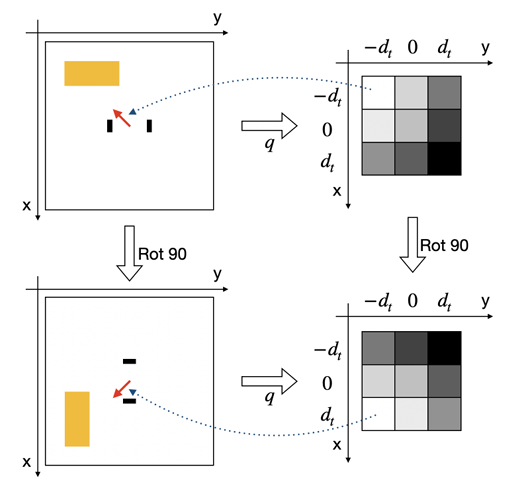
\includegraphics[width=0.95\linewidth]{figures/Q-map_invariance.png}
  \caption{Equivariant DQN $Q$-function. The input depth map (left) is passed through a steerable CNN $q$ to produce a $3 \times 3$ spatial output where each cell scores one planar action $a_{xy}$; rotating the input by $90^{\circ}$ permutes the cells by the same rotation so $Q^{*}$ is $C_4$-invariant jointly in $(s, a_{xy})$. Adapted from \citet{wang2022so2}.}
  \label{fig:dqn-arch}
\end{figure}

\subsection{Equivariant SAC}
Equivariant SAC is continuous-action, so the symmetry is encoded directly into the actor and critic rather than into a gridded output. \citet{wang2022so2} use $C_8$ (eight evenly spaced rotations, finer than DQN's $C_4$) and build an eight-layer equivariant actor $\pi_\theta$ together with an invariant twin critic $(Q_{\phi_1}, Q_{\phi_2})$.

The actor outputs a mean action $\bar a = (a_{xy}, a_{\text{inv}}, \sigma)$. Here $a_{xy} \in \mathbb{R}^2$ is the planar end-effector displacement, which transforms under the standard representation $\rho_1$. The pair $(a_{\text{inv}}, \sigma)$ contains the invariant action components (gripper open/close, vertical displacement, rotation about the vertical axis) together with the policy's per-dimension log-standard-deviation, both transforming under the trivial representation $\rho_0$. The final layer of the actor emits one $\rho_1$ output and several $\rho_0$ outputs, which makes $\pi_\theta(g \cdot s) = g \cdot \pi_\theta(s)$ hold by construction.

\begin{figure}[!tb]
  \centering
  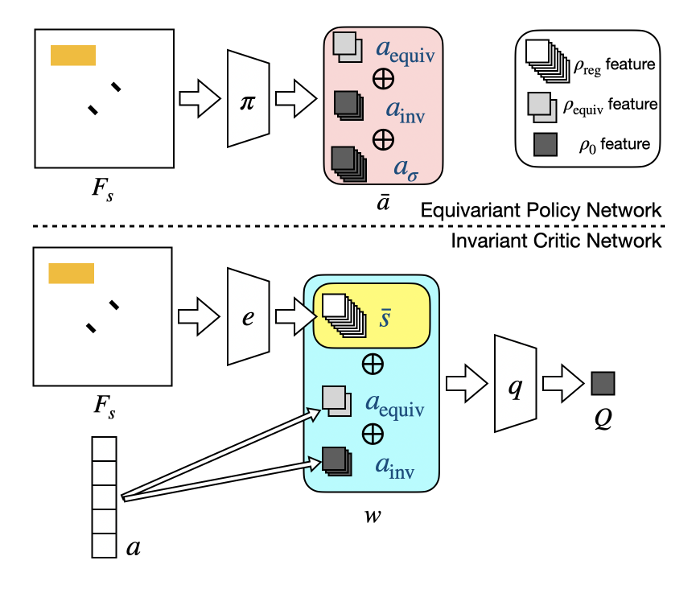
\includegraphics[width=0.95\linewidth]{figures/eq_sac.png}
  \caption{Equivariant SAC architecture. The actor $\pi$ emits one $\rho_1$-typed output $a_{\text{equiv}}$ (planar end-effector displacement), several $\rho_0$-typed outputs $a_{\text{inv}}$ (gripper, vertical displacement, rotation about the vertical axis), and the per-dimension log-standard-deviations $a_{\sigma}$. The critic $q$ encodes the state with an equivariant CNN $e$ to a regular-representation feature $\bar s$, concatenates it with representation-tagged action slots, and reduces to a single invariant scalar $Q$. Adapted from \citet{wang2022so2}.}
  \label{fig:sac-arch}
\end{figure}

The critic $Q_\phi(s, a)$ has to be $C_n$-invariant jointly in its state and action arguments. Wang et al.\ build it by first encoding the state with an equivariant CNN whose output is a regular-representation ($\rho_\text{reg}$) feature vector, concatenating this with a representation-tagged copy of the action (the $\rho_1$ component of the action fills a $\rho_1$ slot, the invariant components fill $\rho_0$ slots), and then passing the result through equivariant layers that reduce to a single invariant scalar. Collapsing the regular representation to the trivial representation needs a non-linear operation, specifically a group-pooling $\max$ across the $n$ cyclic channel copies, rather than a linear projection. The paper shows in its Appendix~B that a linear collapse would over-constrain the $Q$-function to the form $Q(s,a) = \sum_i v_i(s,a)$ and silently lose representational power. The non-linear group-pooling avoids this. The twin critics share the same architecture and are Polyak-averaged to their target copies as in standard SAC.

We match the paper's $C_8$ group, the $\rho_0 / \rho_1 / \rho_\text{reg}$ decomposition at the action and feature-map interfaces, and the non-linear group-pooling in the critic. The SAC losses and optimization schedule from Section~3.1 are used unchanged, with the paper's hyperparameters (Appendix~F of \citealp{wang2022so2}).

\section{Experiments}

\subsection{Experimental Setup}
All experiments follow \citet{wang2022so2}'s close-loop protocol: $20{,}000$ training steps, five-episode evaluation every $500$ environment steps, and a replay buffer pre-loaded with $20$ expert episodes from a hand-coded planner. Hyperparameters are taken from Appendix~F of the paper for SAC and Table~8 (Section~6.1) for DQN; in particular, SAC uses $\gamma = 0.99$, $\tau = 0.01$, and initial temperature $\alpha_0 = 0.01$, while DQN uses $\gamma = 0.95$, batch size $32$, and step sizes $|A_{xy}| = 0.05\,\mathrm{m}$, $|A_z| = 0.02\,\mathrm{m}$, $|A_\theta| = \pi/16$. We report the mean discounted evaluation return with $\pm 1$ standard-deviation bands over two random seeds. Each training run uses five parallel PyBullet environments for collection on a laptop-class NVIDIA RTX~3000 Ada GPU ($8$~GB VRAM).

\begin{figure*}[t]
  \centering
  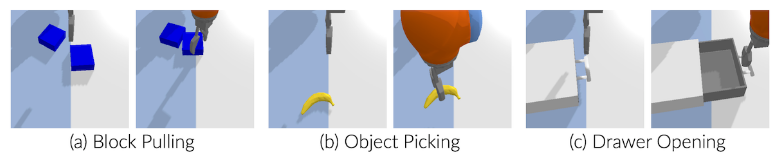
\includegraphics[width=\textwidth]{figures/env_panel_screenshot.png}
  \caption{The three PyBullet close-loop manipulation tasks used throughout our PyBullet experiments: block pulling, block picking (SAC) / object picking (DQN), and drawer opening. Each rollout is initialized with a random object pose and a gripper-centered top-down depth camera is used as the observation.}
  \label{fig:env_panel}
\end{figure*}

\subsection{Equivariant SAC on PyBullet}
Equivariant SAC was evaluated against CNN SAC, DrQ SAC, and FERM SAC on three BulletArm tasks: block pulling, block picking, and drawer opening. Block picking was used in place of the paper's object-picking task because our SAC sweep was locked in early and no household-object SAC runs were completed before the scope freeze. Block picking is the sparse-reward cube variant of the same grasp-and-lift problem.

Learning curves are shown in Figure~\ref{fig:sac-curves}. Equivariant SAC reached a discounted evaluation reward of approximately $0.93$ on all three tasks within about $2{,}500$ training steps and held that plateau for the remaining $17{,}500$ steps. The early convergence is a product of the expert buffer, the $C_8$ equivariance constraint, and an online $SO(2)$ replay augmentation, each of which contributes sample-efficiency on its own. The $20$ pre-loaded expert episodes give the agent a starting distribution of successful trajectories, the equivariance constraint implicitly multiplies each of those episodes by the $8$ rotations in the group, and the online $SO(2)$ buffer adds four rotated copies per transition collected during training. The non-equivariant baselines did not learn block picking or drawer opening and stayed within $[0, 0.05]$ across all $20{,}000$ steps. DrQ partially learned block pulling and reached approximately $0.47$ by the end of training, consistent with the paper's result. CNN and FERM stayed near zero on that task. Our FERM implementation is partially crippled by the omission of the $1{,}600$-step contrastive pre-training phase used by \citet{zhan2020ferm}; the InfoNCE loss is instead applied concurrently with SAC training.

\begin{figure*}[!tb]
  \centering
  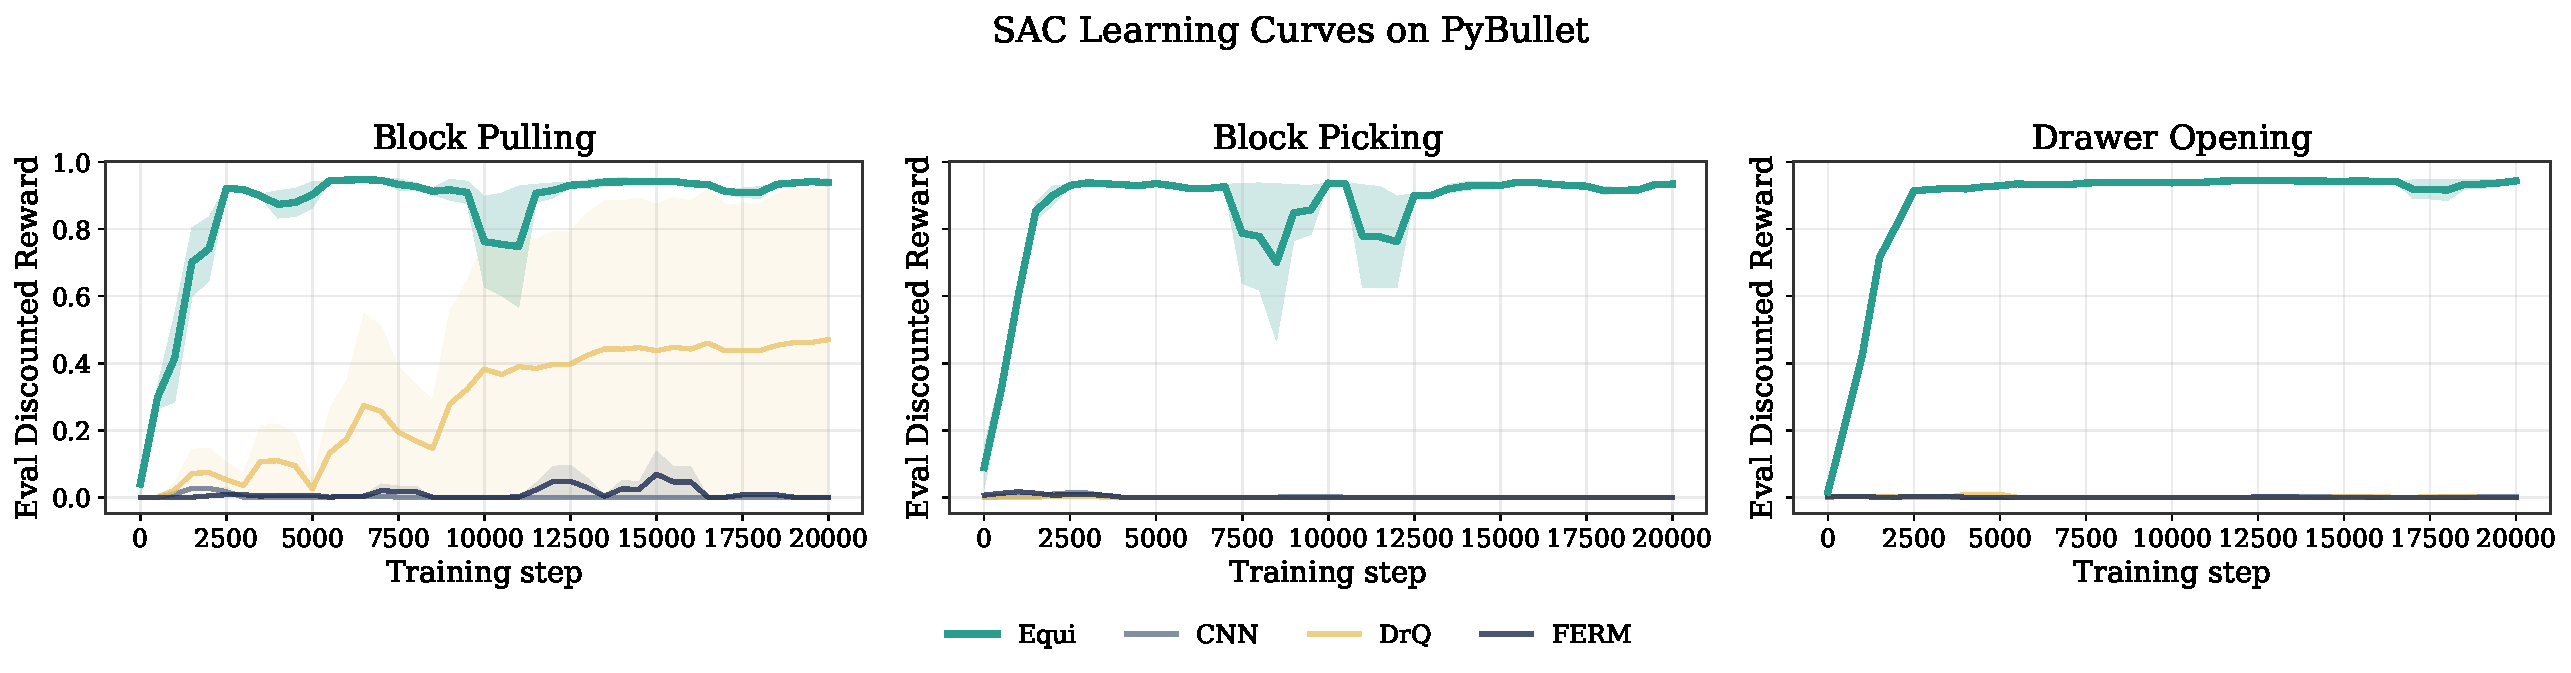
\includegraphics[width=\textwidth]{figures/fig1_sac_bulletarm.pdf}
  \caption{Comparison of Equivariant SAC (teal) with the CNN, DrQ, and FERM baselines on the close-loop BulletArm tasks. The plots show the evaluation performance of the greedy policy in terms of the discounted reward. Evaluation is performed every $500$ training steps. Results are averaged over two seeds; shading denotes standard deviation. Curves are smoothed with a three-point rolling mean.}
  \label{fig:sac-curves}
\end{figure*}

\subsection{Equivariant DQN on PyBullet}
Equivariant DQN was evaluated against CNN DQN, DrQ DQN, and CURL DQN on block pulling, object picking (PyBullet's household-object grasp-and-lift task, i.e.\ Wang et al.\ Figure~6(b)), and drawer opening. Results are shown in Figure~\ref{fig:dqn-curves}. On block pulling, Equivariant DQN led at convergence with a discounted eval return of approximately $0.20$, compared to $0.05$–$0.10$ for CNN, DrQ, and CURL. On object picking, Equivariant DQN reached approximately $0.50$, ahead of the data-augmentation baselines ($0.30$–$0.40$), which themselves were well above random. On drawer opening, where time and compute budget allowed only a single seed per variant, Equivariant DQN and CNN DQN were statistically indistinguishable and both reached approximately $0.45$. The equivariance advantage on DQN was visible but smaller than on SAC at this step budget, matching the trend in the paper's Figure~6: Equivariant DQN outperforms its baselines by a narrower margin than Equivariant SAC does.

\begin{figure*}[!tb]
  \centering
  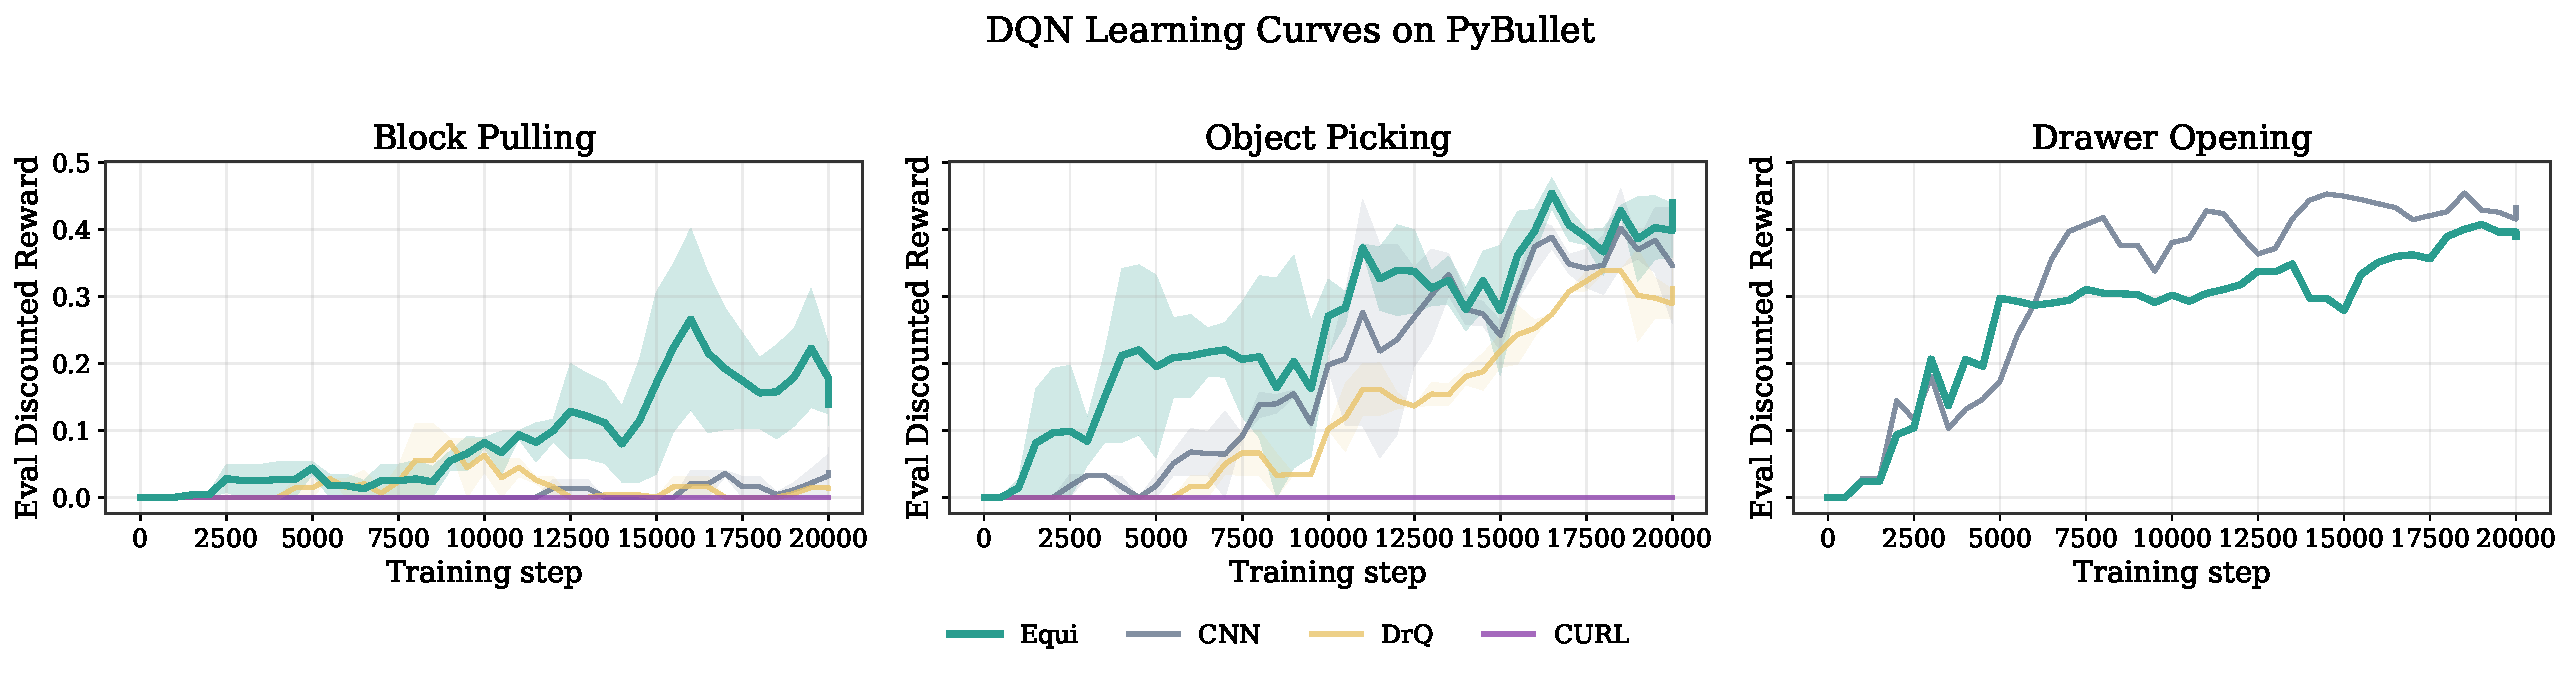
\includegraphics[width=\textwidth]{figures/fig2_dqn_bulletarm.pdf}
  \caption{Comparison of Equivariant DQN with the CNN, DrQ, and CURL baselines on the close-loop PyBullet tasks. The plots show the evaluation performance of the greedy policy in terms of the discounted reward. Evaluation is performed every $500$ training steps. Results are averaged over two seeds for block pulling and object picking, and a single seed for drawer opening; shading denotes standard deviation. Curves are smoothed with a three-point rolling mean.}
  \label{fig:dqn-curves}
\end{figure*}

\subsection{Extension to ManiSkill 3}
The algorithms were ported from PyBullet to ManiSkill~3 \citep{maniskill3}, a GPU-parallel manipulation simulator built on SAPIEN, as a novel extension to the paper. Both IsaacLab and ManiSkill were considered; ManiSkill~3 was chosen because its image-observation pipeline is better documented and because its GPU-batched simulation replaces the CPU multi-processing used in the paper's PyBullet sweeps, trading a dependency on SAPIEN's CUDA kernels for single-process GPU throughput of approximately $42$ SAC steps per second and $370$ DQN steps per second, compared to $\sim 4$ SAC steps per second on PyBullet.

The observation and action spaces were chosen to replicate those of the paper. ManiSkill~3's default sensors did not include an overhead, gripper-aligned camera, so a custom sensor configuration was registered that places a top-down $128 \times 128$ depth camera above the workspace. \texttt{PickCube-v1} was subclassed into \texttt{EquiPickCube-v1} to render the robot arm invisible in the depth stream, which removes the non-equivariant arm geometry that would otherwise be visible in the observation. Only the fingers of the gripper were left visible. This allows the target object to be constantly observed and supports transitional equivariance in the observation. The \texttt{pd\_ee\_delta\_pose} control mode was used so that the action space is a relative end-effector displacement, matching the paper's factored action space. Training ran with $5$ GPU-batched environments per process, replacing the $5$ CPU processes used on PyBullet.

% The four SAC variants (Equi, CNN, DrQ, FERM) and the four DQN variants (Equi, CNN, DrQ, CURL) were then run on PickCube-v1, the ManiSkill~3 task closest to the paper's object-picking setup, with two seeds each and ManiSkill's default \texttt{normalized\_dense} reward.
Due to computational constraints, only CNN SAC was evaluated as a baseline in the ManiSkill environment. Equivariant SAC and CNN SAC were both run on the \texttt{EquiPickCube-v1} environment and evaluated over a set of four trials. Results are shown in Figure~\ref{fig:ms3-sac}.

\begin{figure}[!tb]
  \centering
  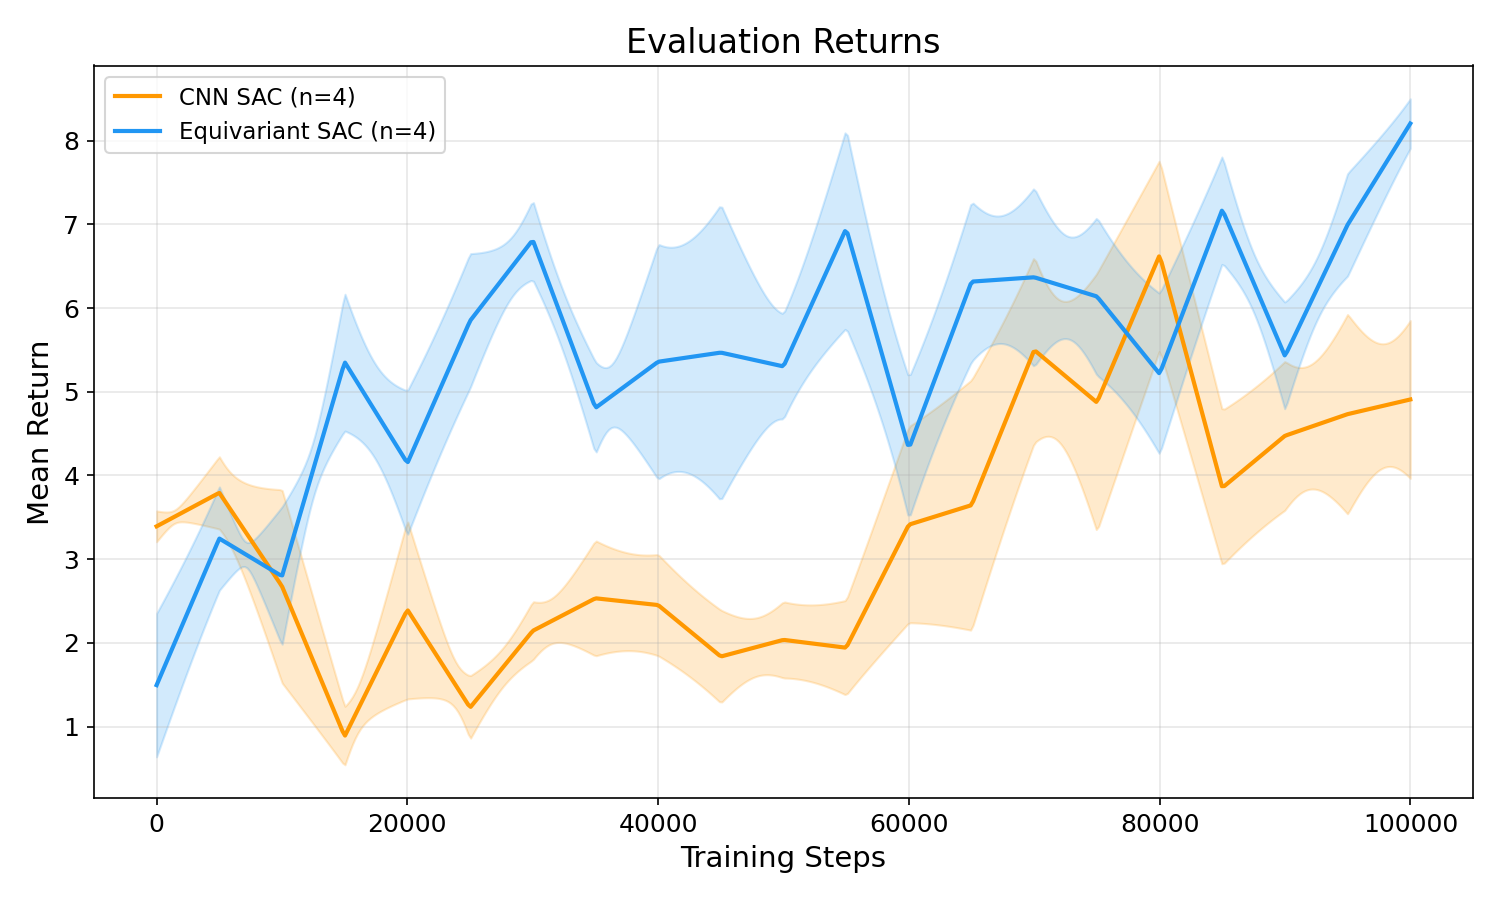
\includegraphics[width=\linewidth]{figures/maniskill_avg_returns.png}
  \caption{ManiSkill~3 EquiPickCube-v1 episodic returns over 4 Trials. Uses a top down observation with hidden arm links. Normalized dense rewards are used as default in the ManiSkill~3 PickCube-v1 environment. }
  \label{fig:ms3-sac}
\end{figure}

% All four SAC variants on ManiSkill~3 PickCube-v1 converged to similar discounted returns in the $2$–$4$ range, and all four DQN variants converged in the $1$–$2$ range. The large sample-efficiency gap visible on BulletArm did not appear here, which is consistent with the paper's framing that equivariance matters most when the baseline has no gradient to follow. BulletArm's sparse $+1$ terminal reward denies the baselines any learning signal until they accidentally succeed, so the implicit $8\times$ expert-demonstration multiplier provided by equivariance is what separates success from no learning. ManiSkill's \texttt{normalized\_dense} reward, by contrast, provides a shaped distance-and-grasp signal at every step, so every variant can make steady progress whether or not it is equivariant. This interpretation was checked by running Equivariant SAC on PickCube-v1 with sparse reward: at $500$ eval steps the agent had reached a discounted reward of $0.00$ and a success rate of $0.00$, with every evaluation episode hitting the $100$-step timeout. This is the same ``no-gradient'' regime that forces equivariance to pay off on BulletArm. A sparse-reward MS3 comparison at a larger step budget (on the order of $100{,}000$ to $500{,}000$ env steps, consistent with typical PickCube-v1 training schedules) is therefore the natural next experiment to carry the paper's contribution into the new simulator.

\section{Challenges}

Porting the equivariant pipeline from PyBullet to a GPU-parallel simulator was not a smooth process. The PyBullet environments used in the original paper were custom-built for equivariance and expose an observation that no existing manipulation simulator provides by default: a depth image rendered from a virtual camera that tracks the gripper's horizontal position, points straight down, and covers a fixed physical area of the workspace regardless of gripper height, with the robot arm hidden from the render. This rig is not a reasonable physical camera and was not a convenience option in ManiSkill. It was approximated in ManiSkill by registering a top-down overhead camera through the simulator's sensor configuration interface, and by subclassing PickCube-v1 to render the robot arm invisible so that the arm geometry does not enter the depth image. The depth values were then clipped and centered so that their range matches the PyBullet observation. This observation-space mismatch was the biggest source of debugging time in the ManiSkill port.

Compute was the other hard constraint. The experiments in this report were run on a single laptop-class $8$~GB GPU, with a small amount of additional throughput from a shared lab machine. Runs on the lab machine were kept conservative so that they would not exhaust the GPU memory shared with another user, and the training budget was limited to $20{,}000$ steps per run at two seeds per variant rather than the four seeds used by the paper. The shared lab machine also uses an NVIDIA Blackwell-generation GPU, and the SAPIEN physics binaries shipped with our ManiSkill install do not yet support that architecture. A debug pass was attempted and was deferred so that the shared environment would not be destabilized.

A few small details cost time to track down. DQN's $xy$ step size has to match between the expert planner and the discrete action grid used at decode time. An off-by-$0.03$\,m between the two silently corrupts the replay buffer, since the stored grid index no longer matches the physical motion in the simulator. The paper's augmentation baselines use shift for DrQ and crop for CURL, and FERM at specific pixel budgets, not the $SO(2)$ rotation augmentation we started with. The PyBullet single-runner also needs an explicit auto-reset flag between evaluation episodes, which is not set by default. Without it, every eval episode after the first runs a single step and the eval statistics collapse to a uniform episode length of $10.8$. All three were caught in the two days before submission.

With more time, the project could have been extended in several directions. A larger compute budget would have allowed four seeds per variant, matching the paper's evaluation. The FERM SAC baseline would have been re-run with the $1{,}600$-step contrastive pre-training phase described in \citet{zhan2020ferm}, rather than the concurrent InfoNCE loss used here. The ManiSkill extension would have been scaled to block pulling and drawer opening so that the PyBullet-to-ManiSkill comparison covers the full task set, and a full sparse-reward ManiSkill comparison would have been run at a training budget on the order of $100{,}000$ to $500{,}000$ env steps in order to reproduce the PyBullet sample-efficiency pattern in the new simulator. Resolving the SAPIEN-on-Blackwell kernel incompatibility would have also unlocked the shared lab machine for that larger budget.

\section{Conclusion}

The main result of \citet{wang2022so2} was reproduced on three PyBullet close-loop manipulation tasks. Under sparse reward and a small number of expert demonstrations, equivariance was the difference between learning and not learning for SAC. Equivariance was also an advantage for DQN, although smaller and slower to emerge. The paper's architectural claim, that enforcing $C_n$-equivariance in the policy and $C_n$-invariance in the $Q$-function is both sufficient and far more sample-efficient than learning the same symmetry from data, held up in our reimplementation at two seeds per variant.

The ManiSkill~3 extension also worked. Equivariant and non-equivariant SAC and DQN now run on a GPU-parallel simulator with a gripper-aligned depth observation, scripted expert demonstrations, prioritization, and online $SO(2)$ buffer augmentation, all ported from the PyBullet pipeline. Under ManiSkill's default dense rewards, Equivariant SAC had a significant improvement over vanilla CNN based SAC, but neither was able to effectively learn to complete the task. This result suggests that equivariance is most useful in environments with constrained observational inputs, and that it does not guarantee efficient policy learning.
% Under ManiSkill's default shaped reward the four variants converged to similar returns, which matches the paper's point that equivariance matters most when the baselines have no gradient to follow. A brief sparse-reward sanity check on PickCube-v1 reproduced the ``no-signal'' starting condition and supports that read.

Our reimplementation of the paper's PyBullet sweeps and the ManiSkill~3 extension is available at \url{https://github.com/wade-g-williams/so2_equi_rl} and \url{https://github.com/joeyhz/eq_sac}.

\bibliography{references}

\end{document}
